\documentclass{article}
\usepackage[utf8]{inputenc}
\usepackage{polski}
\usepackage{graphicx}
\usepackage{fancyhdr}
\usepackage{lastpage}
\usepackage{listings}
\usepackage{hyperref}
\usepackage[T1]{fontenc}


\pagestyle{fancy}

\fancyhf{}

\fancyfoot[C]{\thepage\ / \pageref{LastPage}} % Ustawienie numeracji stron w stopce

\fancypagestyle{plain}{ % Nadpisanie stylu strony tytułowej
    \fancyhf{}
    \renewcommand{\headrulewidth}{0pt} % Usunięcie nagłówka
    \fancyfoot[C]{\thepage\ / \pageref{LastPage}}
}

\title{Specyfikacja implementacyjna projektu 2\linebreak w języku Java}
\author{Miłosz Mertka i Sebastian Grosfeld}
\date{\today}

\lstdefinestyle{tree}{
    literate=
    {├}{{\smash{\raisebox{-1ex}{\rule{1pt}{\baselineskip}}}\raisebox{0.5ex}{\rule{1ex}{1pt}}}}1 
    {─}{{\raisebox{0.5ex}{\rule{1.5ex}{1pt}}}}1 
    {└}{{\smash{\raisebox{0.5ex}{\rule{1pt}{\dimexpr\baselineskip-1.5ex}}}\raisebox{0.5ex}{\rule{1ex}{1pt}}}}1 
  }

\begin{document}

\maketitle

\tableofcontents

\newpage

% Poniżej ustawiany jest nagłówek
\setlength{\headheight}{23pt}
\lhead{Miłosz Mertka\\Sebastian Grosfeld}
\rhead{Sprawozdanie końcowe\\projektu 2 w języku Java}

\section{Wprowadzenie}

Celem projektu jest stworzenie programu, który będzie w stanie wykonać następujące zadania:
\begin{enumerate}
    \item Wygeneruje graf w postaci siatki (\emph{Rysunek \ref{fig:wagi}}) o podanej liczbie kolumn i wierszy. Krawędzie i wagi krawędzi losowane są w podanym zakresie wartości.
    \item Zapisze taki graf do pliku o ustalonym formacie.
    \item Przeczyta z pliku o ustalonym formacie taki graf.
    \item Potrafi określić za pomocą algorytmu BFS, czy dany graf jest spójny.
    \item Potrafi wyznaczyć w tym grafie najkrótsze ścieżki pomiędzy wybranymi parami wierzchołków, korzystając z algorytmu Dijkstry.
\end{enumerate}
\begin{figure}[htp]
        \centering
        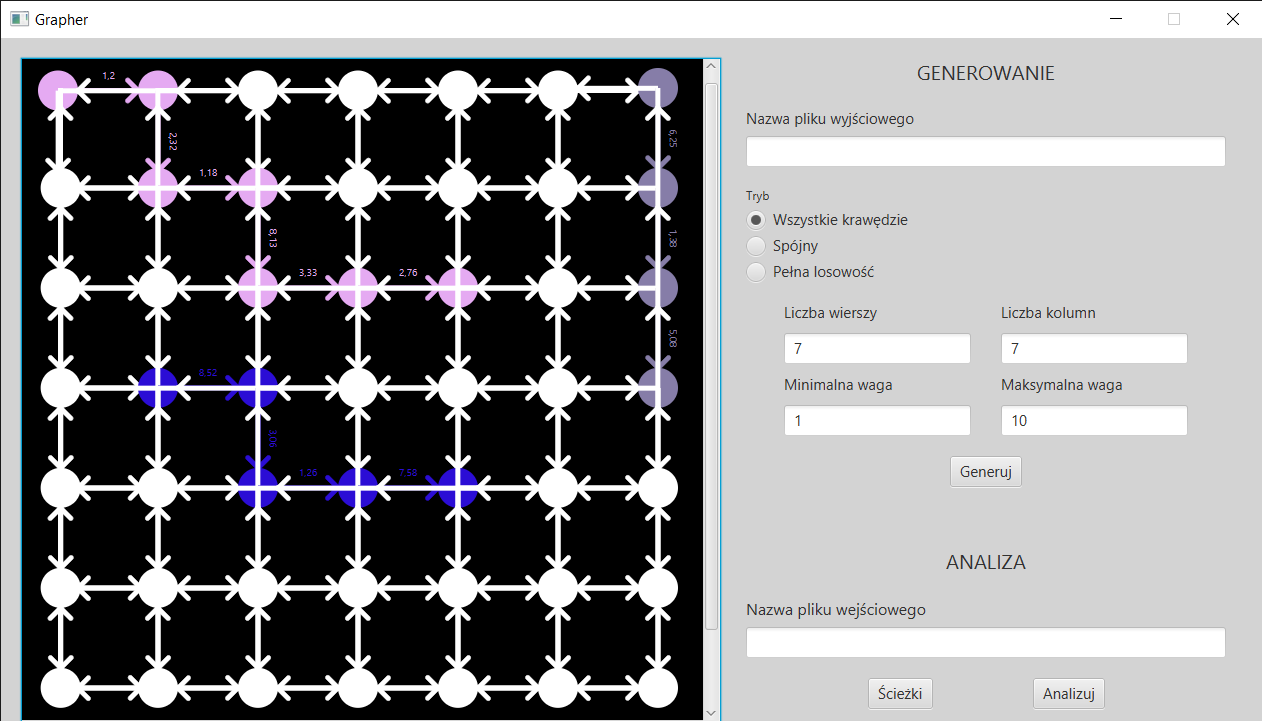
\includegraphics[width=11cm]{Images/MainScene.png}
        \caption{Okno główne programu}
        \label{fig:wagi}
\end{figure}
\textbf{Graf} definiuje się następująco: $G=(V,E)$. $V$ jest zbiorem wierzchołków grafu, $E$ jest zbiorem jego krawędzi.
\vspace{5mm}
\\
\textbf{Algorytm BFS} nazywany jest algorytmem \emph{przeszukiwania grafu wszerz}.\linebreak W projekcie znajduje on zastosowanie przy sprawdzaniu, czy dany graf jest spójny.
\vspace{5mm}
\\
\textbf{Algorytm Dijkstry} służy do wyznaczania najkrótszych ścieżek od wierzchołka źródłowego do wszystkich innych wierzchołków grafu. Algorytm działa wyłącznie dla grafów ważonych, którego wagi są nieujemne. W projekcie narzucony został także dodatkowy wymóg spójności danego grafu, aby mieć pewność,\linebreak że algorytm Dijkstry znajdzie zadane ścieżki.

\section{Aktualny stan projektu}
\subsection{Struktura katalogów}

W katalogu \emph{test} znajduje się \emph{test\textunderscore files} zawierający pliki wykorzystywane \linebreak w testach (ich opis został zawarty w \emph{Specyfikacji funkcjonalnej projektu 2 \linebreak w języku Java}, która znajduje się w pliku \emph{Specyfikacja\textunderscore funkcjonalna\textunderscore Java.pdf}). W tym samym katalogu zostały zawarte testy jednostkowe aplikacji. 

Poniżej struktura dla \textbf{grapher/src}.

\begin{lstlisting}[style=tree]
.
├───main
│ └───java
│  │ └───org
│  │  │└───grapher
│  │  │  │├───gui
│  │  │  │ │├───AnalizationSettings.java
│  │  │  │ │├───EdgeComponent.java
│  │  │  │ │├───ErrorAlert.java
│  │  │  │ │├───GenerationSettings.java
│  │  │  │ │├───GraphView
│  │  │  │ │├───InformationAlert.java
│  │  │  │ │├───MainScene.java
│  │  │  │ │├───NodeComponent.java
│  │  │  │ │└───PathsScene.java
│  │  │  │├───logic
│  │  │  │ │├───BFS.java
│  │  │  │ │├───Dijkstra.java
│  │  │  │ │├───Edge.java
│  │  │  │ │├───FileHandler.java
│  │  │  │ │├───Graph.java
│  │  │  │ │├───Node.java
│  │  │  │ │└───Path.java
│  │  │  │└───main
│  │  │  │ │└───Main.java
└───test
│ ├───java
│  │ └───org
│  │  │└───grapher
│  │  │  │└───logic
│  │  │  │ │├───EdgeTest.java
│  │  │  │ │├───GraphTest.java
│  │  │  │ │├───NodeTest.java
│  │  │  │ │└───PathTest.java
│ └───test_files
│  │ ├───cos_graph.txt
│  │ ├───incos_graph.txt
│  │ ├───t_graph.txt
│  │ ├───wf_graph.txt
\end{lstlisting}

Poszczególne pakiety zostały opisane poniżej:
\begin{itemize}
    \item \textbf{main} - zawiera główną klasę z metodą \textbf{main()};
    \item \textbf{gui} - zawiera klasy odpowiedzialne za wyświetlanie oraz interakcję użytkownika z graficznym interfejsem programu;
    \item \textbf{logic} - zawiera klasy odpowiedzialne za wewnętrzną logikę programu;
\end{itemize}

\subsection{Diagram klas}
Na stronie poniżej został ukazany diagram klas dla projektu (\emph{Rysunek \ref{fig:g7}})



\begin{figure}[htp]
        \centering
        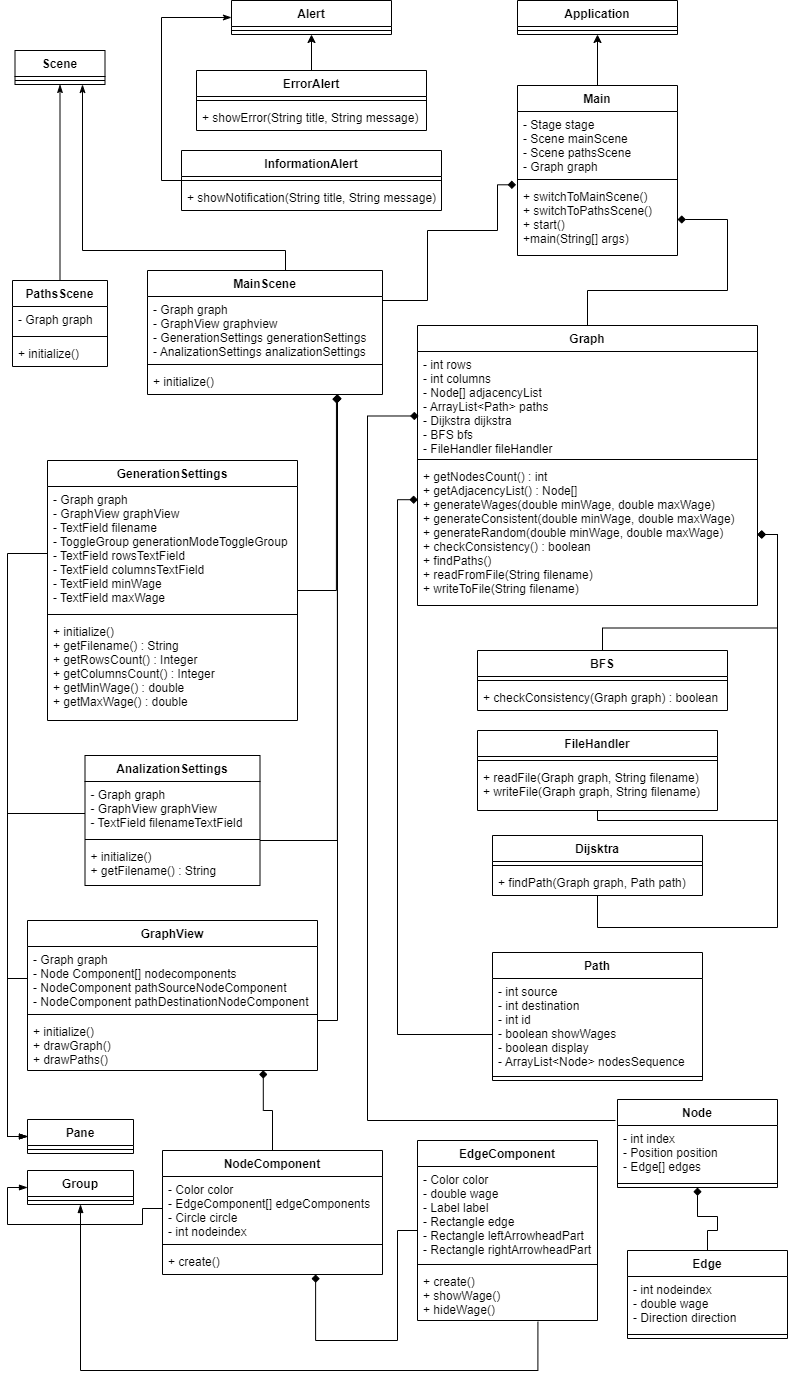
\includegraphics[width=9cm]{Images/diagramklas.png}
        \caption{Diagram klas dla projektu}
        \label{fig:g7}
    \end{figure}
\newpage

Opis poszczególnych klas na diagramie został umieszczony poniżej.
\begin{itemize}
    \item \textbf{Main} -- wejście do programu. Startuje aplikacją i przechowuje referencje do scen i grafu.
    
    Atrybuty:
    \begin{itemize}
        \item \textbf{Stage stage} -- okno aplikacji,
        \item \textbf{Scene mainScene} -- główna scena aplikacji,
        \item \textbf{Scene pathsScene} -- scena edycji ścieżek,
        \item \textbf{Graph graph} -- referencja do obiektu reprezentującego graf.
    \end{itemize}
    
    Metody:
    \begin{itemize}
        \item \textbf{switchToMainScene()} -- przełącza do głównej sceny programu,
        \item \textbf{switchToPathsScene()} -- przełącza do sceny edycji ścieżek,
        \item \textbf{start()} -- inicjalizuje aplikację,
        \item \textbf{main(String[ ] args)} -- stanowi wejście do programu.
    \end{itemize}
    
    \item \textbf{ErrorAlert} -- statyczna klasa służąca do pokazywania komunikatów\linebreak o błędach.
    
    Metody:
    \begin{itemize}
        \item \textbf{showError(String title, String message)} -- pokazuje alert o zadanym tytule i treści.
    \end{itemize}
    
    \item \textbf{PathsScene} -- klasa stanowiąca scenę do zarządzania ścieżkami.
    
    Atrybuty:
    \begin{itemize}
        \item \textbf{Graph graph} -- referencja do obiektu reprezentującego graf.
    \end{itemize}
    
    Metody:
    \begin{itemize}
        \item \textbf{initialize()} -- inicjalizuje scenę.
    \end{itemize}
    
\newpage
    
    \item \textbf{MainScene} -- klasa stanowiąca scenę główną programu.
    
    Atrybuty:
    \begin{itemize}
        \item \textbf{Graph graph} -- referencja do obiektu reprezentującego graf,
        \item \textbf{GraphView graphView} -- referencja do obiektu reprezentującego sekcję GUI z narysowanym grafem,
        \item \textbf{Settings generationSettings} -- referencja do obiektu reprezentującego sekcję GUI z opcjami do generowania grafu,
        \item \textbf{Settings analizationSettings} -- referencja do obiektu reprezentującego sekcję GUI z opcjami do analizowania grafu.
    \end{itemize}
    
    Metody:
    \begin{itemize}
        \item \textbf{initialize()} -- inicjalizuje scenę.
    \end{itemize}
    
    \item \textbf{AnalizationSettings} -- klasa stanowi reprezentację sekcji z opcjami\linebreak do analizowania grafu.
    
    Atrybuty:
    \begin{itemize}
        \item \textbf{Graph graph} -- referencja do obiektu reprezentującego graf,
        \item \textbf{GraphView graphView} -- referencja do obiektu reprezentującego sekcję GUI z narysowanym grafem,
        \item \textbf{TextField filenameTextField} -- referencja do obiektu reprezentującego pole tekstowe z nazwą pliku wejściowego.
    \end{itemize}
    
    Metody:
    \begin{itemize}
        \item \textbf{initialize()} -- inicjalizuje sekcję,
        \item \textbf{getFilename() : String} -- zwraca nazwę pliku wpisaną do pola tekstowego.
    \end{itemize}
    
    \item \textbf{InformationAlert} -- statyczna klasa służąca do pokazywania komunikatów informacyjnych.
    
    Metody:
    \begin{itemize}
        \item \textbf{showNotification(String title, String message)} -- pokazuje alert o zadanym tytule i treści.
    \end{itemize}
    
\newpage
    
    \item \textbf{GenerationSettings} -- klasa stanowi reprezentację sekcji z opcjami\linebreak do generowania grafu.
    
    Atrybuty:
    \begin{itemize}
        \item \textbf{Graph graph} -- referencja do obiektu reprezentującego graf,
        \item \textbf{GraphView graphView} -- referencja do obiektu reprezentującego sekcję GUI z narysowanym grafem,
        \item \textbf{TextField filenameTextField} -- referencja do obiektu reprezentującego pole tekstowe z nazwą pliku wyjściowego,
        \item \textbf{ToggleGroup generationModeToggleGroup} -- referencja do obiektu reprezentującego grupę pól typu radio, które służą do wyboru trybu generowania grafu,
        \item \textbf{TextField rowsTextField} -- referencja do obiektu reprezentującego pole tekstowe z liczbą wierszy,
        \item \textbf{TextField columnsTextField} -- referencja do obiektu reprezentującego pole tekstowe z liczbą kolumn,
        \item \textbf{TextField minWageTextField} -- referencja do obiektu reprezentującego pole tekstowe z minimalną wagą krawędzi,
        \item \textbf{TextField maxWageTextField} -- referencja do obiektu reprezentującego pole tekstowe z maksymalną wagą krawędzi.
    \end{itemize}
    
    Metody:
    \begin{itemize}
        \item \textbf{initialize()} -- inicjalizuje sekcję,
        \item \textbf{getFilename() : String} -- zwraca nazwę pliku wpisaną do pola tekstowego,
        \item \textbf{getRowsCount() : int} -- zwraca liczbę wierszy wpisaną do pola tekstowego,
        \item \textbf{getColumnsCount() int} -- zwraca liczbę kolumn wpisaną do pola tekstowego,
        \item \textbf{getMinWage() : double} -- zwraca minimalną wagę krawędzi wpisaną do pola tekstowego,
        \item \textbf{getMaxWage() : double} -- zwraca maksymalną wagę krawędzi wpisaną do pola tekstowego.
    \end{itemize}
    
\newpage
    
    \item \textbf{GraphView} -- klasa stanowi reprezentację sekcji z widokiem wczytanego lub wygenerowanego grafu.
    
    Atrybuty:
    \begin{itemize}
        \item \textbf{Graph graph} -- referencja do obiektu reprezentującego graf,
        \item \textbf{NodeComponent[ ] nodecomponents} -- pole reprezentujące wierzchołki grafu (GUI),
        \item \textbf{NodeComponent pathSourceNodeComponent} -- pole reprezentujące wierzchołek będący początkiem ścieżki,
        \item \textbf{NodeComponent pathDestinationNodeComponent} -- pole reprezentujące wierzchołek będący końcem ścieżki.
    \end{itemize}
    
    Metody:
    \begin{itemize}
        \item \textbf{initialize()} -- inicjalizuje sekcję,
        \item \textbf{drawGraph()} -- rysuje graf na podstawie jego definicji,
        \item \textbf{drawPaths()} -- rysuje ścieżki na podstawie ich definicji.
    \end{itemize}
    
    \item \textbf{NodeComponent} -- klasa stanowi reprezentację wierzchołka grafu (GUI).
    
    Atrybuty:
    \begin{itemize}
        \item \textbf{Color color} -- pole przechowujące kolor wierzchołka,
        \item \textbf{EdgeComponent[ ] edgeComponents} -- pole reprezentujące krawędzie wychodzące z danego wierzchołka (GUI).
    \end{itemize}
    
    Metody:
    \begin{itemize}
        \item \textbf{create(Node node)} -- tworzy graficzną reprezentację danego wierzchołka grafu.
    \end{itemize}
    
    \item \textbf{EdgeComponent} -- klasa stanowi reprezentację wierzchołka grafu (GUI).
    
    Atrybuty:
    \begin{itemize}
        \item \textbf{Color color} -- pole przechowujące kolor krawędzi,
        \item \textbf{double wage} -- wartość wagi krawędzi,
        \item \textbf{Label Label} -- referencja do obiektu reprezentującego etykietę z napisem zawierającym wartość wagi krawędzi.
        \item \textbf{Rectangle edge} -- krawędź
        \item \textbf{Rectangle leftArrowheadPart} -- lewy grot krawędzi
        \item \textbf{Rectangle rightArrowheadPart} -- prawy grot krawędzi
    \end{itemize}
    
    Metody:
    \begin{itemize}
        \item \textbf{create()} -- tworzy graficzną reprezentację danej krawędzi grafu,
        \item \textbf{showWage()} -- wyświetla wagę dla krawędzi,
        \item \textbf{hideWage()} -- ukrywa wagę dla krawędzi.
    \end{itemize}
    
\newpage
    
    \item \textbf{Graph} -- klasa stanowi reprezentację grafu.
    
    Atrybuty:
    \begin{itemize}
        \item \textbf{int rows} -- liczba wierszy grafu,
        \item \textbf{int columns} -- liczba kolumn grafu,
        \item \textbf{Node[ ] adjacencyList} -- graf przechowywany jako lista sąsiedztwa,
        \item \textbf{ArrayList$<$Path$>$ paths} -- lista przechowująca ścieżki,
        \item \textbf{BFS bfs} -- referencja do obiektu implementującego algorytm BFS,
        \item \textbf{Dijkstra dijkstra} -- referencja do obiektu implementującego algorytm Dijkstry,
        \item \textbf{FileHandler fileHandler} -- referencja do obiektu obsługującego zapis i odczyt plików.
    \end{itemize}
    
    Metody:
    \begin{itemize}
        \item \textbf{getNodesCount() : int} -- zwraca liczbę wierzchołków grafu,
        \item \textbf{generateWages(double minWage, double maxWage)} -- generuje graf ze wszystkimi krawędziami i wagami losowymi w zadanym przedziale,
        \item \textbf{generateConsistent(double minWage, double maxWage)} -- generuje graf spójny z wagami losowymi w zadanym przedziale,
        \item \textbf{generateRandom(double minWage, double maxWage)} -- generuje graf w pełni losowy z wagami losowymi w zadanym przedziale,
        \item \textbf{checkConsistency()} -- sprawdza spójność grafu,
        \item \textbf{findPaths()} -- szuka najkrótszych ścieżek w grafie na podstawie ich definicji,
        \item \textbf{readFromFile(String filename)} -- wczytuje graf z pliku o zadanej nazwie,
        \item \textbf{writeToFile(String filename)} -- zapisuje graf do pliku o zadanej nazwie.
    \end{itemize}
    
\newpage
    
    \item \textbf{Path} -- klasa opisuje ścieżkę między dwoma wierzchołkami grafu.
    
    Atrybuty:
    \begin{itemize}
        \item \textbf{Integer source} -- numer wierzchołka źródłowego,
        \item \textbf{Integer destination} -- numer wierzchołka docelowego,
        \item \textbf{int id} -- numer identyfikacyjny ścieżki,
        \item \textbf{boolean showWages} -- czy pokazywać wagi dla przejść między wierzchołkami grafu,
        \item \textbf{boolean display} -- czy wyświetlać ścieżkę,
        \item \textbf{ArrayList$<$int$>$ nodesSequence} -- sekwencja numerów wierzchołków od wierzchołka źródłowego do docelowego.
    \end{itemize}
    
    \item \textbf{FileHandler} -- klasa służąca do obsługi plików.
    
    Metody:
    \begin{itemize}
        \item \textbf{readFile(Graph graph, String filename)} -- wczytuje graf z pliku o zadanej nazwie,
        \item \textbf{writeFile(String filename, Graph graph)} -- zapisuje dany graf do pliku o zadanej nazwie.
    \end{itemize}
    
    \item \textbf{BFS} -- klasa służąca do analizy grafu pod kątem spójności.
    
    Metody:
    \begin{itemize}
        \item \textbf{checkConsistency(Graph graph) : boolean} -- analizuje spójność grafu z wykorzystaniem algorymtu BFS.
    \end{itemize}
    
    \item \textbf{Dijkstra} -- klasa służąca do wyszukiwania najkrótszej ścieżki między zadanymi wierzchołkami w grafie.
    
    Metody:
    \begin{itemize}
        \item \textbf{findPath(Graph graph, Path path)} -- wyszukuje najkrótszą ścieżkę w grafie dla zadanych wierzchołków przy użyciu algorymtu Dijkstry.
    \end{itemize}
    
    \item \textbf{Node} -- klasa stanowiąca reprezenatację wierzchołka.
    
    Atrybuty:
    \begin{itemize}
        \item \textbf{int index} -- index wierzchołka,
        \item \textbf{Position position} -- pozycja wierzchołka,
        \item \textbf{Edge[] edges} -- reprzezentacja krawędzi wierzchołka.
    \end{itemize}
    
    \item \textbf{Edge} -- klasa stanowiąca reprezenatację krawędzi.
    
    Atrybuty:
    \begin{itemize}
        \item \textbf{int nodeIndex} -- index krawędzi,
        \item \textbf{double wage} -- waga krawędzi,
        \item \textbf{Direction direction} -- położenie względem wierzchołka.
    \end{itemize}
\end{itemize}

\subsection{Instrukcja uruchomienia}
Program został zbudowany razem z zależnościami do pliku \emph{grapher.jar}. Dzięki temu (będąc
w katalogu z tym plikiem) możemy go uruchomić prostym poleceniem:

\medskip
\textbf{java -jar grapher.jar}

\subsection{Obsługa programu}
Obsługa programu została zawarta w \emph{Specyfikacji funkcjonalnej projektu 2 \linebreak w języku Java} w pliku \emph{Specyfikacja\textunderscore funkcjonalna\textunderscore Java.pdf}

\subsection{Wymagania funkcjonalne}
Program potrafi:
\begin{itemize}
    \item wygenerować i wyświetlić graf o podanej liczbie kolumn i wierszy, z krawędziami o wagach z przedziału określonego minimalną i maksymalną wagą, w określonym trybie generacji; 
    \item wyznaczyć najkrótsze ścieżki między podanymi wierzchołkami, jeśli graf jest spójny i zaznaczyć je na wyświetlonym grafie;
    \item zapisać wygenerowany graf do pliku o podanej nazwie i w określonym formacie;
    \item odczytać graf z pliku o podanej nazwie, zanalizować ten graf pod względem spójności oraz wyświetlić go. 
\end{itemize}

\subsection{Wymagania niefunkcjonalne}
Program:
\begin{itemize}
    \item jest napisany w języku Java;
    \item możliwe jest jego uruchomienie z poziomu konsoli;
    \item program jest budowany przy użyciu Maven-a.
\end{itemize}

\subsection{Testowanie}
Kod jest testowany za pomocą automatycznych testów jednostkowych (JUnit). Wszystkie pliki potrzebne przy testowaniu znajdują się w katalogu \linebreak \textbf{grapher/src/test}. Testy sprawdzają poprawność:
\begin{itemize}
    \item generowania grafu w określonych trybach;
    \item wyznaczania najkrótszych ścieżek w grafie;
    \item zapisu grafu do pliku w ustalonym formacie;
    \item odczytu grafu z pliku w ustalonym formacie.
\end{itemize}

\section{Przykłdowe wyniki}
Poniżej znajdują się przykładowe wyniki działania programu.

\begin{itemize}
    \item Graf z wszytkimi krawędziami o wymiarach 4x4, wagi krawędzi od 2 do 7 jest zapisywany do pilku \emph{graf1}.
    \begin{figure}[htp]
        \centering
        \includegraphics[width=11cm]{Images/wages4x4&2-7.png}
        \caption{Wygenrowany graf z wszystkimi krawędziami}
        \label{fig:g1}
    \end{figure}
    
    \newpage
    
    \item Graf spójny o wymiarach 2x2, wagi krawędzi od 3 do 4 jest zapisywany do pliku \emph{graf2}.

    \begin{figure}[ht]
        \centering
        \includegraphics[width=11cm]{Images/cos2x2&3-4.png}
        \caption{Wygenrowany graf spójny}
        \label{fig:g2}
    \end{figure}
    
    Zawartość pliku \emph{graf2}:
    \begin{lstlisting}
2 2
	 1 :3.8218646545337966  2 :3.349934275174142  
	 3 :3.9341340318753684  
	 0 :3.147245477617951  
	 2 :3.212974575444834 
    \end{lstlisting}
    
    \newpage
    
    \item Graf w pełni losowy o wymiarach 3x6, wagi krawędzi od 2 do 9, nie jest zapisywany do pliku.
    
     \begin{figure}[ht]
        \centering
        \includegraphics[width=11cm]{Images/ran3x6&2-9.png}
        \caption{Wygenrowany graf losowy}
        \label{fig:g3}
    \end{figure}
    
    \newpage
    
    \item Graf wczytany z pliku testowego \emph{incos\textunderscore graph}.
    
    \begin{figure}[ht]
        \centering
        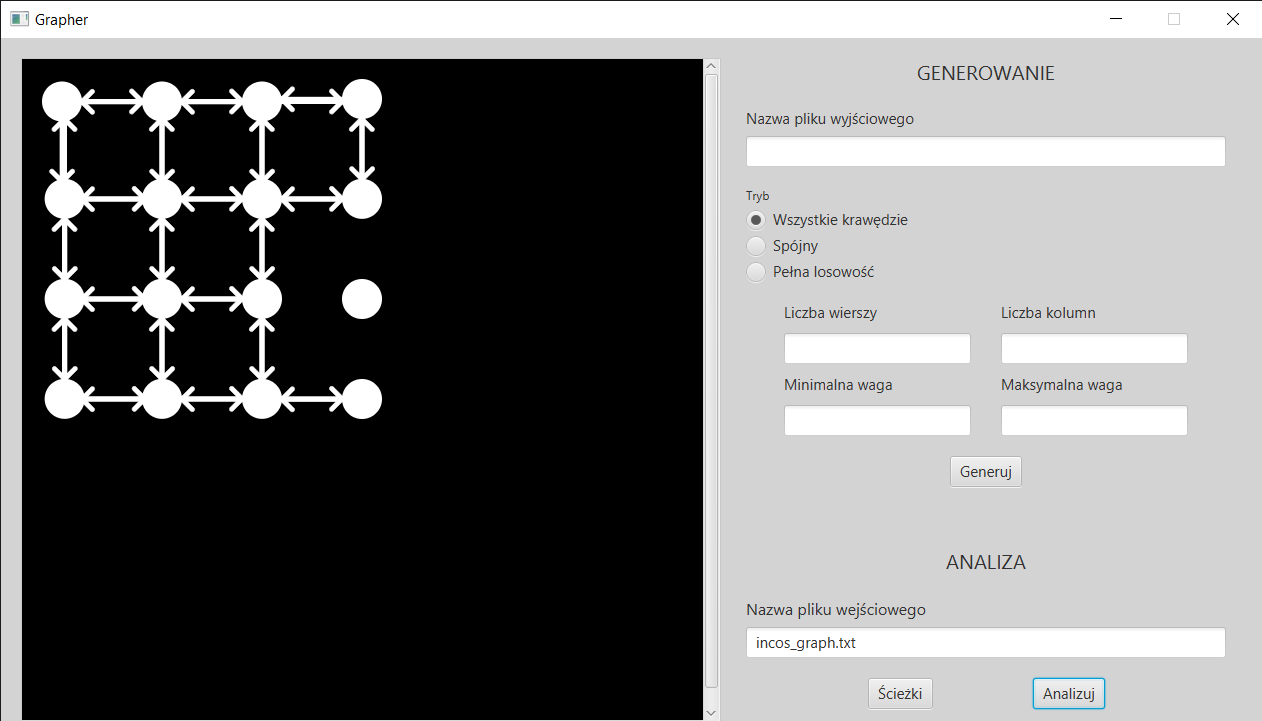
\includegraphics[width=11cm]{Images/analize.png}
        \caption{Wczytany graf}
        \label{fig:g4}
    \end{figure}
    
    Dodatkowo pojawił się komunikat informujący o spójności.
    
    \begin{figure}[ht]
        \centering
        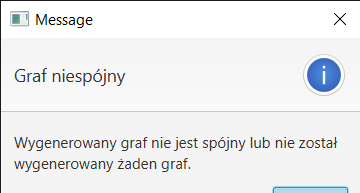
\includegraphics[width=7cm]{Images/Message.png}
        \caption{Komunikat}
        \label{fig:g4}
    \end{figure}
    
\end{itemize}

\newpage
\section{Lista zmian}
Poniżej zostały opisane zmiany w projekcie względem specyfikacji. 

\begin{itemize}
    \item Została usunięta klasa abstrakcyjna \textbf{Settings}.
    \item Została dodana klasa \textbf{InformationAlert} obsługująca komunikaty informacyjne.
    \item Przebudowano klasy \textbf{Node} i \textbf{Edge}, teraz obie odpowiadają za logikę programu. Za wierzchołki i krawędzie w odniesieniu do GUI odpowiadają nowe klasy, \textbf{NodeComponent} za wierzchołki i \textbf{EdgeComponent} za krawędzie.
    \item Uległ zmanie sposób przechowywania listy sąsiedztwa w klasie \textbf{Graph}. Zamiast tablicy dwuwymiarowej typu \textit{double} zastosowano tablicę jednowymiarową \textbf{Node-ów}, gdzie każdy Node zawiera tablicę \textbf{Edge-ów}.
    \item Minimalna ilość wierszy dla generowanego grafu została zmieniona z 0 na 2.
    \item Minimalna ilość kolumn dla generowanego grafu została zmnieniona z 0 na 2.
    \item Metody \textbf{getRowsCount} i \textbf{getColumnsCount} w klasie \textbf{GenerationSettings} zwracają teraz obiekt klasy \textbf{Integer}.
\end{itemize}

\section{Współpraca podczas projektu}
Współpraca podczas prac nad projektem składała się na regularne spotkania członków zespołu, podczas których wymieniali się poglądami, wizją oraz pomysłami związanymi z zagadnieniami projektowymi, a także wspólnie pracowali nad dokumentacją i kodem. Jej drugą częścią było wspólne pracowanie na repozytorium oraz wzajemna kontrola kodu. Dowodem na to są chociażby commity widoczne w logach w zdalnym repozytorium.

\section{Podsumowanie projektu i wnioski końcowe}
Podczas wspólnej pracy nad projektem, jako członkowie zespołu, rozwinęliśmy umiejętności skutecznej współpracy nad projektem programistycznym\linebreak w zespole. Zyskaliśmy szersze doświadczenie w pracy ze zdalnym repozytorium\linebreak oraz nauczyliśmy się efektywnie rozplanowywać czas pracy. W trakcie prac poszerzyliśmy swoje umiejętności programistyczne w języku Java oraz nauczyliśmy się pisać aplikacje z graficznym interfejsem użytkownika przy pomocy biblioteki JavaFX, zapoznaliśmy się z Maven-em oraz obsługą testów jednostkowych przy pomocy JUnit. Projekt pozwolił także zapoznać się z aspektami programowania obiektowego i nauczyć się stosowania pewnych zalecanych dobrych zasad pisania kodu.
Jeśli mielibyśmy coś zmienić w projekcie, to z pewnością zaczęlibyśmy wcześniej pracę nad kodem. Wynika to z implementacji interfejsu graficznego, która wydłużyła czas pracy nad projektem w porównaniu z projektem nieposiadającym GUI. Dużym problemem w trakcie pracy nad projektem było przygotowanie środowiska programistycznego (tj. konfiguracja pliku pom.xml, przygotowanie odpowiedniego JDK i konfiguracja testów).
\end{document}
